\documentclass[letterpaper, 12pt]{article}


\usepackage{cmjStyle-pdftex} %use CMJ style
\usepackage{natbib} %natbib package, necessary for customized cmj BibTeX style
\bibpunct{(}{)}{;}{a}{}{,} %adapt style of references in text

% \doublespacing


\raggedright % use this to remove spacing and hyphenation oddities
%\setlength{\parindent}{0} % first para indent?
\setlength{\parskip}{2ex}
\parindent 24pt
\urlstyle{same} % make url tags have the same font
\setcounter{secnumdepth}{-1} % remove section numbering

\usepackage{ifpdf}

\DeclareGraphicsExtensions{.pdf,.png,.jpg}
\graphicspath{{../fig/}}


%% The package endfloat moves all floats (figures, tables...) to the end of the paper, as required for the final version of a CMJ paper.
%% Leave this package commented out for initial submission, but uncomment it for final version. 

 \usepackage{endfloat}

\usepackage{microtype}


%---Document----------
\begin{document}

{\cmjTitle 	Computation as material: (meta) live coding experiences}
\vspace*{24pt}

% (In the initial submission, omit all the following author information to ensure anonymity during peer review.)

%author - name
{\cmjAuthor Till Bovermann}
%author - address
\newline
\begin{cmjAuthorAddress}
	Media Lab Helsinki, Department of Media\\
	Aalto University\\
	H\"ameentie 135 c\\
	00560 Helsinki, Finland\\
	till.bovermann@aalto.fi
\end{cmjAuthorAddress}

\vspace*{24pt}
{\cmjAuthorPhone +358 (50) 5296398}
\vspace*{24pt}

%author - name
{\cmjAuthor Dave Griffiths}
%author - address
\newline
\begin{cmjAuthorAddress}
	FoAM\\
	Koolmijnenkaai 30-34\\
	1080 Brussels\\
	Belgium\\
	dave@fo.am
\end{cmjAuthorAddress}

\vspace*{24pt}
{\cmjAuthorPhone +32 2 5135928}
\vspace*{24pt}


% use of asterisk in section number to remove numbering
\section{Abstract}


% Analog to the Audio Sniffer.\footnote{\url{http://www.openmusiclabs.com/projects/audio-sniffer/}}
 % In difference to the above-mentioned \emph{Spork factory} approach that introduced  new instructions to facilitate signal generation

\subsection{Unfolding self modification to livecode pseudo-collaboration} 
\label{sec:unfolding_self_modification_to_livecode_collaboration}



At it's core, Betablocker provides a simple virtual machine for playing with music which is 'unstoppable' (any combination of instructions can be executed). It started off originally as a Fluxus scheme program, then got rewritten in C++ for the Nintendo DS, and has now been ported to Supercollider. I've built yet another Linux commandline version, and glued it to the Java Genetic Algorithms Package via Clojure.

This means I can continue with the genetic programming experiments and try evolving programs using a real genetic algorithm framework, using the betablocker instruction set. This is mainly just for kicks, but it's also partly to "grow" new strategies for livecoding betablocker and researching instruction sets more generally.
The first test was to try and find a program to just play note 99. I would write this in betablocker like this (using a text representation of the icon interface for convenience):

\begin{Verbatim}[fontfamily=courier, xleftmargin=\parindent]
   pshl 99 ; push the literal value 99 on to the stack
   note    ; play the top of the stack as a note 
\end{Verbatim}

First we need a fitness function to score the results from the programs which are generated:

\begin{Verbatim}[fontfamily=courier, xleftmargin=\parindent]
(defn fitness [notes]
    (- 255 (Math/abs (- (first notes) 99))))
\end{Verbatim}

It takes a list of the notes played by a candidate program, and measures how far away the first element is from 99 - the bigger the number, the fitter the individual program is. I gave it 8 instructions to work with and a population of 500 individuals - after just a couple of generations, this chromosome/program popped up with a top fitness of 255 - meaning it was successfully playing note 99:

\begin{Verbatim}[fontfamily=courier, xleftmargin=\parindent]
99 46 213 89 7 142 23 168
\end{Verbatim}

Which when disassembled looks something like this:
\begin{Verbatim}[fontfamily=courier, xleftmargin=\parindent]
    99       ; <-- address 0 
    nop
    nop
    nop
    pshi 142 ; pushes contents of address at location 142 (which is 0)
    note     ; play the note
    nop
\end{Verbatim}

This program has grown taking advantage of the fact that the memory is initialised to zero, so if it dereferences a large address like 142 it will be zero and load the contents of the first byte - 99. It's this kind of wacked out approach genetic algorithms are great at finding/abusing.
The next problem, something a bit more general - create a sequence of notes which are all different to one another. The fitness function:

\begin{Verbatim}[fontfamily=courier, xleftmargin=\parindent]
(defn list-contains? [l i]
  (cond
   (empty? l) false
   (= (first l) i) true
   :else (recur (rest l) i)))

(defn fitness [a]
  (count
   (reduce
    (fn [r v]
      (if (not (list-contains? r v))
        (cons v r)
        r))
    '()
    a)))
\end{Verbatim}

This just counts the number of unique elements in the list - again, the higher the better. This one took longer, but eventually came up with this:  

\begin{Verbatim}[fontfamily=courier, xleftmargin=\parindent]
139 246 1 23 12 22 23 12 20 95 22 3
\end{Verbatim}

Which when disassembled:

\begin{Verbatim}[fontfamily=courier, xleftmargin=\parindent]
    nop
    nop
    org
start:
    note      ; play a note
    inc       ; increment top stack byte
    dup       ; duplicate top stack byte
    note      ; play a note (consumes 1 stack byte)
    inc       ; increment again
    pip 95    ; increment address 95 (junk - doesn't have any effect)
    dup       ; duplicate again
    jmp start ; return to the start
\end{Verbatim}

Which plays a rising sequence of notes, with none repeated, so the highest fitness achievable:

\begin{Verbatim}[fontfamily=courier, xleftmargin=\parindent]
0 1 2 3 4 5 6 7 8 9 10 11 12 13 14 15 16 17 18 19 20 21
\end{Verbatim}

This is already doing much better than the genetic programming I was mucking about with before - indeed there seems to be some literature on evolving java bytecode, but with betablocker there is an advantage that you don't need to enforce the correctness of the programs before they can be run.


Following on from the first BetaBlocker genetic algorithm bytecode experiments, in addition to the "most different notes" fitness function I added a similar calculation for the first derivative (ie. the difference between the notes in time order). This was an attempt to steer the evolution away from simple scales and into more complex patterns.

\begin{Verbatim}[fontfamily=courier, xleftmargin=\parindent]
(defn deriv [l]
  (cond
   (empty? l) '()
   (empty? (rest l)) '()
   :else (cons (- (first (rest l)) (first l))
               (deriv (rest l)))))
\end{Verbatim}
	       
The code to find the first derivative of a sequence of notes - eg. (deriv '(1 2 3 2 6 7)) => (1 1 -1 4 1). We then add this to the fitness function which looks like this:

\begin{Verbatim}[fontfamily=courier, xleftmargin=\parindent]
(+ (count (num-unique res)) ; unique notes are good
   (count (num-unique (deriv res))) ; unique gaps between notes are good
   (min (count res) 20)) ; lots of notes are good (stop at 20)
\end{Verbatim}
   
This resulted in the following bytecode to emerge from the primordial soup: 23 17 7 6 23 21 9 23 8 212 3 2 4 2 180 124 - which disassembles to:

\begin{Verbatim}[fontfamily=courier, xleftmargin=\parindent]
	note      ; stack is empty, so plays zero
	not       ; pushes bitwise "not" of zero => 255
loop:
	pshi 6    ; push the contents of address 6 (-> 9 = 212)
	note      ; play the note (212)
	pdp 9     ; decrement address 9 (212 becomes 211)
	note      ; plays 255 first time, 0 after that when stack is empty
	pop 212   ; stack is now empty so writes 0 to adress 212
	jmp loop  ; goto loop
	jmpz 2    ; junk, we never reach here
	nop
	nop
\end{Verbatim}

The arrows show the indirection which helps as this one is a bit tricky to pull apart. It's the first time I've seen self modification emerge - it decrements the "212" and uses it as a variable for the note sequence. Combining the pshi and pdp like this is a nice trick I can make use of when programming betablocker myself.
The program is self destructive - the "pop" which otherwise does nothing of use will eventually write zeros over the program itself if it's run for a few more cycles than the 100 I'm testing the programs for.
The output looks like this: 

\begin{Verbatim}[fontfamily=courier, xleftmargin=\parindent]
0 212 255 211 0 210 0 209 0 208 0 207 0 206 0 205 0 204 0 203 0 202 0 201 0 200 0 199 0 198 0 197 0 196
\end{Verbatim}

According to our fitness function, the interleaved zeros give it a very high scoring derivative list:

\begin{Verbatim}[fontfamily=courier, xleftmargin=\parindent]
212 43 -44 -211 210 -210 209 -209 208 -208 207 -207 206 -206 205 -205 204 -204 203 -203 202 -202 201 -201 200 -200 199 -199 198 -198 197 -197 196
\end{Verbatim}

However the actual pattern is not so interesting, so still more work needed on the fitness criteria.

For the next attempt in BetaBlocker bytecode evolution I wanted to favour patterns that had a rhythmic nature by measuring them with this function:

\begin{Verbatim}[fontfamily=courier, xleftmargin=\parindent]
(defn freq [l n]
  (defn _ [c]
    (cond
     (>= (+ c n) (count l)) 0
     (= (nth l c) (nth l (+ c n))) (+ 1 (_ (+ c 1)))
     :else (_ (+ c 1))))
  (_ 0))
\end{Verbatim}

Which looks for repeating values spaced apart by "n" positions, so (freq '(100 1 2 3 100 4 5 6 100 7 8 9 100) 4) returns 3, as it finds 3 pairs of equal values (100) distanced by the specified 4 positions.
With this fitness function:

\begin{Verbatim}[fontfamily=courier, xleftmargin=\parindent]
(+ (* 50 (count (num-unique res))) ; unique notes are very good
   (freq res 4) ; equal notes every 4 beats are good
   (freq res 6)) ; equal notes every 6 beats are good
\end{Verbatim}

We favour rhythmic components of 4 or 6 beats and boost the uniqueness score by multiplying it by 50. After some generations, we get a high scoring individual: 23 23 13 22 7 12 17 20 12 23 23 5 0 7 12 3 
Which disassembles as:

\begin{Verbatim}[fontfamily=courier, xleftmargin=\parindent]
loop:
    note    ; play & remove top of stack (zero when empty)
    note    ; play & remove top of stack
    dec     ; decrement top of stack
    dup     ; duplicate - pushes a copy of stack top 
    pshi 12 ; push the value pointed at by address at 12 (self read)
    not     ; performs bitwise not on stack top
    pip 12  ; increment value at address 12
    note    ; play & remove top of stack
    note    ; play & remove top of stack
    pshl 0  ; pushes this literal number (the 0 is at address 12)
    pshi 12 ; push the value pointed at by 12 (self read)
    jmp loop
\end{Verbatim}
    
This program creates a pattern from 4 separate sources, using all 16 bytes of code:


The result: "0 0 232 255 23 1 232 254 13 2 242 253 22 3 233 252 7 4 248 251 12 5 243 250 17 6 238 249 20 7 235 248 12 8" scores poorly for it's rhythmic patterns, but it's probable that this surprising local maxima was found by the early influence of the rhythmic fitness criteria on it's ancestor populations. 

\subsection{Embedded evolved code} 
\label{sub:embedded}

A system for creating an abundance of useless software for tiny devices. Spork Factory evolves programs that run on Atmel processors, the same make as found on the Arduino, in this case the ATtiny85, a �2.50 8 pin 8bit CPU. I'm currently simply using a piezo speaker as an output and evolving programs based on the frequency of the sound produced by flipping the pins up and down, so creating 2bit synths using the Fourier transform as the fitness function. With more hardware (input as well as output) perhaps we could evolve small robots, or even maybe cheap claytronics or programmable matter experiments.

This project reuses the previous genetic programming experiments (including jgap as its genetic algorithm framework), and is also inspired by Till Bovermann's recent work with Betablocker in Supercollider for bytecode synthesis.

The programs generated don't use the Atmel instruction set directly, but interpret a custom one derived from Betablocker for two reasons. Atmel processors separate their instruction memory from data (the Harvard architecture) which makes it difficult to modify code as it's running (either uploading new evolved code or running self modifying instructions), the other is that using a simplified custom instruction set makes it easier for genetic algorithms to create all kinds of strange programs that will always run.

I've added an 'OUT' instruction, which pops the top of the stack and writes it to the pins on the ATtiny, so the first thing a program needs to do is generate and output some data. The second thing it needs to do is create an oscillator to create a tone, after that the fitness function grades the program on the amount of frequencies present in the sound, encouraging it to make richer noises.

Here are two example programs from a single run, first the ancestor, a simple oscillator which evolved after 4 or 5 generations:

\begin{Verbatim}[fontfamily=courier, xleftmargin=\parindent]
    out
    out
    nop
    nop
    dec
    nop
    nop
    nop
    out
    nop
    jmpz 254
    nop
    nop
    nop
    dup
\end{Verbatim}

It's simply outputting 0's, then using the 'dec' to decrement the top of the stack to make a 255 which sets the rightmost bit to 1 (the one the speaker is attached to) and then loops with the 'jmpz' causing it to oscillate. This program produces this fft plot:

\begin{figure}
	\centering
		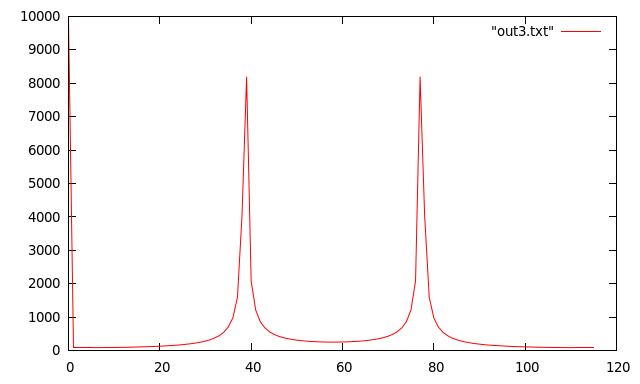
\includegraphics[width=13cm]{spork1}
	\caption{XOR rave}
	\label{fig:fig_spork1}
\end{figure}

After 100 or so further generations, this descendant program emerges. The dec is replaced by \u2018pshl 81\u2032 which does the same job (pushes the literal value 81 onto the stack, setting our speaker bit to 1) but also uses a \u2018dup\u2019 (duplicate top of the stack) to shuffle the values around to make a more complex output signal with more frequencies present:

\begin{Verbatim}[fontfamily=courier, xleftmargin=\parindent]
loop:
    out
    out
    not
    nop
    pshl 81
    pshi 149
    out
    nop
    out
    nop
    dup
    psh 170
    jmp loop
\end{Verbatim}

\begin{figure}
	\centering
		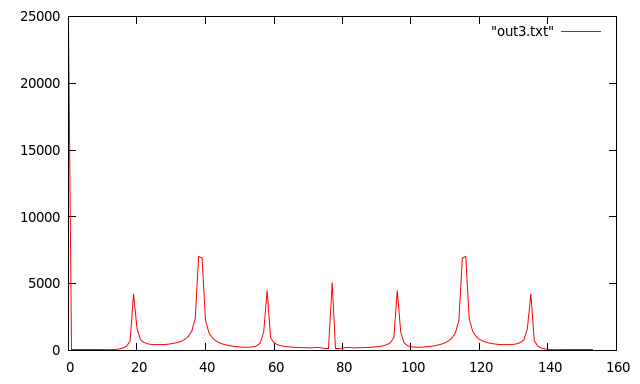
\includegraphics[width=13cm]{spork2}
	\caption{XOR rave}
	\label{fig:fig_spork2}
\end{figure}

Also robotics, an evolved light follower:

\begin{Verbatim}[fontfamily=courier, xleftmargin=\parindent]
    pshl 171 
loop:
    lmot 
    leye 
    pip 111 
    pip 30 
    rmot 
    reye 
    pshl 214 
    nop 
    lmot 
    jmp loop
\end{Verbatim}

\begin{figure}
	\centering
		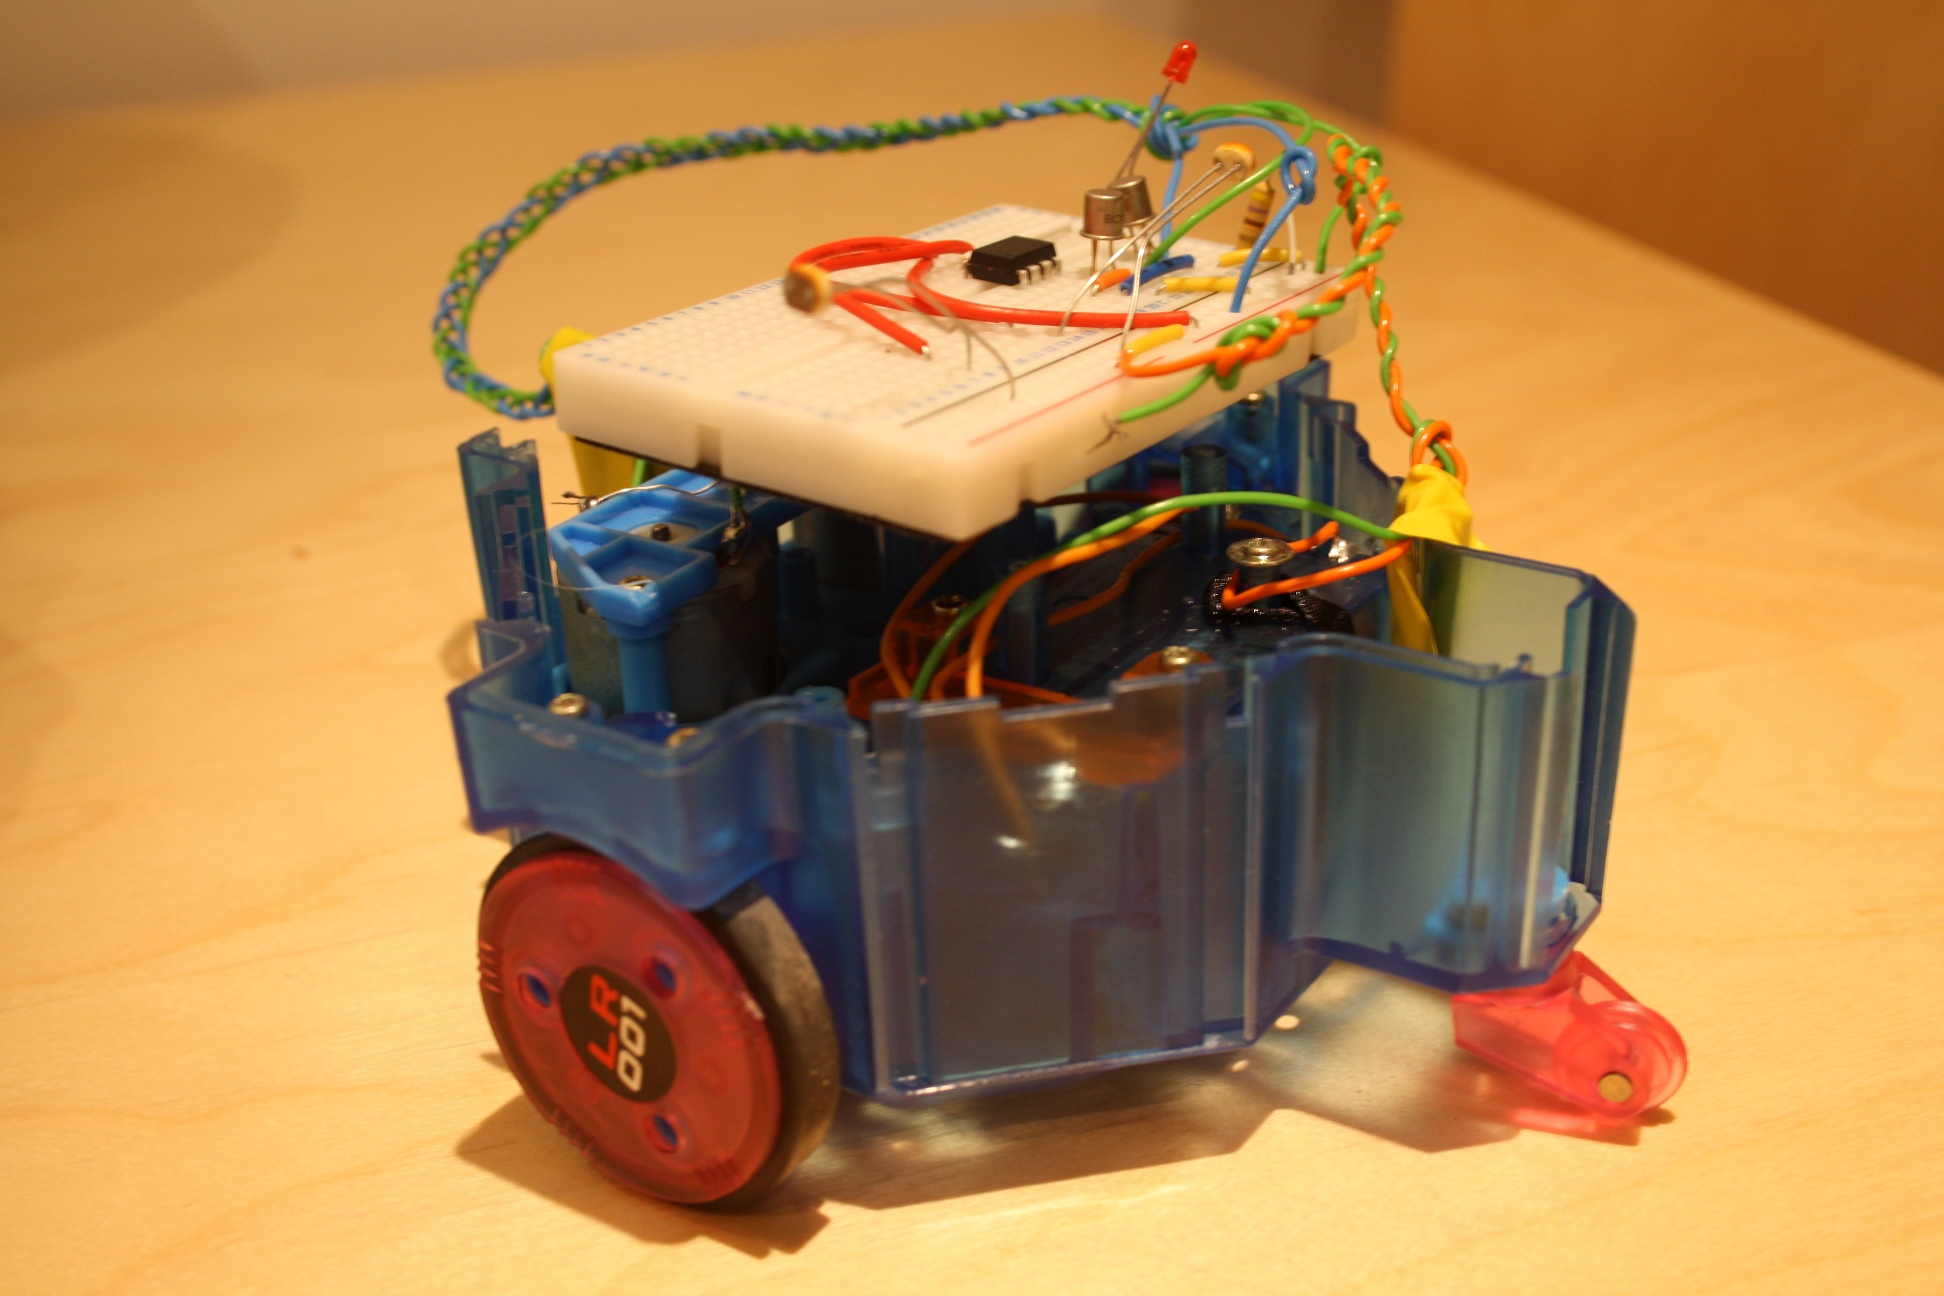
\includegraphics[width=13cm]{bbbot}
	\caption{caption}
	\label{fig:fig_bbbot}
\end{figure}

\subsection{Towards Amorphous livecoding} 
\label{sub:amorphous_livecoding}

\begin{figure}
	\centering
		
\includegraphics[width=13cm]{amorphous}
	\caption{500 betablocker CPUs}
	\label{fig:amorphous}
\end{figure}

Departing in a new direction after evolved light follower robots, take 500 processor cores spread out in space. Give them a simple instruction set which includes a instruction to copy (DMA) 8 bytes of their code/data to nearby cores (with an error rate of 0.5%). Fill the cores with random junk and set them running. If we graph the bandwidth used (the amount of data transmitted per cycle by the whole system) we get a plot like this:
\begin{figure}
	\centering
		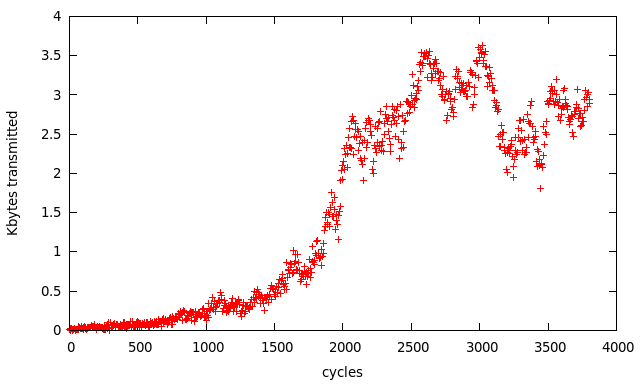
\includegraphics[width=13cm]{amorphous-bandwidth}
	\caption{Bandwidth}
	\label{fig:amorphous-bandwidth}
\end{figure}

This explosion in bandwidth use is due to implicit emergence of programs which replicate themselves. There is no fitness function, it's not a genetic algorithm and there is no guided convergence to a single solution - no 'telling it what to do'. Programs may arise that cooperate with each other or may exhibit parasitic behaviour as in alife experiments like Tierra, and this could be seen as a kind of self modifying, emergent Amorphous computing - and eventually, perhaps a way of evolving programs in parallel on cheap attiny processor hardware.


% pseudo-interaction
%% human (behaviour) <---> computer (pseudo-proactive behaviour)

% a turing-test for livecode companions



\section{Research in computing processes (Till's junkyard)}
\label{sub:research_in_computing_processes}

Based on phenomenological methods/maxims, treating the subject of investigation (here: BetaBlocker) as being only perceivable \emph{through} phenomena (things "present to the mind"). 
As we are interested in sonic qualities, the selected modality of the observed phenomena are mainly of sonic nature.
On our way through the system, though, other introspective as well as extrospective data emerged and was taken into account.

To illustrate the research journey, we will now list key events that happened:

Starting point was a collection of C files that defined the BetaBlocker core.
To keep things simple at the beginning, a crucial strategy in implementations, we decided to fill the heap with a very simple program resembling a sawtooth \texttt{[ORG, INC, JMP, 0]}. 
After successfully listening to this basic setup, we replaced the hardcoded heap with one that gets initialised with random values between $0$ and $255$.\footnote{\url{http://tai-studio.org/index.php/2011/05/betablocker-ugen/}}


Airy, sustained sound clouds; mostly high-pitched broken up occasionally by a rhythmical pattern


\begin{itemize}	 
\item Implemented access to heap's data. This means that it can be set, read and manipulated while running. Also, several engines can share a heap. 
	% http://tai-studio.org/index.php/2011/08/detablockerbuf-8channel/ 
\item helper classes facilitating the generation of BBlocker programs 
	% http://tai-studio.org/index.php/2011/08/twentydblockers/ 
\item further sonic exploration, listening sessions 
	% http://tai-studio.org/index.php/2011/10/betablocker-pieces/

	For now, the layout is always additive, i.e., several BBlocker engines next to each other

\item Idea generation
	% http://tai-studio.org/index.php/2011/10/betablocker-theory-day/ 
\item Visual representation
	% http://tai-studio.org/index.php/2011/11/attempt-for-representing-2x8bit/
\item public demo video
	% http://tai-studio.org/index.php/2011/12/dblockerintro/ 
\item adding convenience methods play/scope/plot to BBlockerProgram based on feedback of first introduction to a non-programmer
	% http://tai-studio.org/index.php/2011/12/cambridge-day-4/ 
\item New iteration of the BetaBlocker wrapper, adding more output (pos and whole stack) and removing the possibility to control it with demand rate,
	% http://tai-studio.org/index.php/2011/12/60-panned/ 
	includes a sound study.
\item Multi-out UGen with audio-rate input
	% http://tai-studio.org/index.php/2011/12/cambridge-day-8/
\item Decision to focus on sonic aspects. Therefore tried to write/design programs with specific sonic features in mind.
	% http://tai-studio.org/index.php/2011/12/cambridge-days-912/
\item FM-like synthesis strategy added
\item Performance at Cambridge, fixed setup
\item Rehearsal for SuperCollider Symposium
\item Concert at SuperCollider Symposium
\item Workshop at UdK.
\item Oulipop performance
\end{itemize}



\section{Meta}
\label{sec:meta}




\vspace*{24pt}





\vspace*{24pt}


% % format for Heading-B style
% \subsection{Format for Heading-B Style; Use This for Subsection Headings}
% 
% Insert body text here.  
% 
% % format for Heading-C style
% \subsubsection{Format for Heading-C Style; Use This for Minor Sub-subsection Headings}
% 
% Insert body text here.
% 
% In the initial manuscript submission, you are encouraged to include figures (with captions) inline with the text, for ease of reading during the review process. For example, like this:
% 
% % include figures in text with captions for initial submission, like this:
% \begin{figure}[htpb]
% \begin{center}
% \includegraphics{myFigure.pdf}
% \caption{Insert Figure caption here.}
% \label{fig:myFigure}
% \end{center}
% \end{figure}
% 
% However, for the final version after the manuscript has been accepted, all figures should be moved to the end so that the text only contain markers like ``[Figure 1 about here]'' near where the figure would normally have occurred. You can rearrange the text to this effect simply by enabling the package {\tt endfloat} as suggested in the header of this document.
% 
% 
% % equations
% You can insert equations inline with the text like this:
% 
% \begin{equation}
% 	\label{radupdate}
% 		\Psi_{N}^{n+1} = m_{N}^{(-)}\Psi_{N-1}^{n}+m_{N}^{(0)}\Psi_{N}^{n} + q_{N}\Psi_{N}^{n-1}
% \end{equation}
% where
% \begin{eqnarray*}
% 	m_{N}^{(-)} &=& \frac{\lambda^2}{2\tau}\left(S_{N+1}+2S_{N}+S_{N-1}\right)\\
% 	m_{N}^{(0)} &=& \frac{1}{\tau}\left(2-\frac{\lambda^2}{2}\left(S_{N+1}+2S_{N}+S_{N-1}\right)\right)\\
% 	q_{N} &=& \frac{1}{\tau}\left(\frac{\gamma^2 k^2}{2h}\left(S_{N+1}+S_{N}\right)\left(\frac{\alpha_{1}}{k}-	\alpha_{2}\right)-1\right)
% \end{eqnarray*}
% and where 
% \begin{equation*}
% 	\tau = \frac{\gamma^2 k^2}{2h}\left(S_{N+1}+S_{N}\right)\left(\frac{\alpha_{1}}{k}+\alpha_{2}\right)+1
% \end{equation*}
% 
% % Use this environment for inserting source code examples.
% % Note, that this will print out text in the document exactly as you type it here in the .tex file. That means you can add empty spaces, tabs, blank lines here and they will be printed out like this in the document.). 
% %For more information check out the LaTeX-Package 'fancyvbr' documentation
% %
% \begin{Verbatim}[fontfamily=courier, xleftmargin=\parindent]
% Use this style for program code, for example:
% main() {
%     printf("Hello World\n");    
% }
% \end{Verbatim}
% 
% %use of references
% Some examples for the use of references in the text:\\
% %author name in sentence, single authors
% \cite{Ano08}, \cite{Bele68}, \cite{Ther99}, \cite{Zica02},
% %author name in sentence, multiple authors
% \cite*{VeRo00}, \cite*{AtDa04}, 
% %reference in brackets, multiple authors
% \citep*{AtDa04} 


%References
\bibliographystyle{cmj}
% \bibliography{cmjbib}
\bibliography{/Users/tboverma/Public/unpub/BibTeX/bovermann}
\end{document}
